% !TeX spellcheck = de_DE
\documentclass[ngerman]{scrartcl} 

\KOMAoptions{fontsize=12pt, paper=a4}
\KOMAoptions{DIV=11}
\usepackage[utf8]{inputenc}             % Direkte Eingabe von ä usw.
\usepackage[T1]{fontenc}               	% Font Kodierung für die Ausgabe
\usepackage{babel}                   	% Verschiedenste sprach-spezifische Extras
\usepackage{parskip}
\usepackage[autostyle=true]{csquotes}	% Intelligente Anführungszeichen
\usepackage{amsmath}					% Mathematischer Formelsatz mit zusätzlichen mathematischen Schriften und Symbolen
\usepackage{amssymb}					% Mathematischer Formelsatz mit zusätzlichen mathematischen Schriften und Symbolen
\usepackage{physics}					% Differentialgleichungen
\usepackage{listings}					% Zum Einbinden von Programmcode verwenden wir das listings-Paket
\usepackage[dvipsnames]{xcolor}			% um Elemente von Befehlen farblich zu unterstützen
\usepackage[varg]{txfonts}              % Schönere Schriftart
\usepackage{graphicx}					% Paket um externe Graphiken einzufügen
\usepackage{media9}
\RequirePackage[backend=biber, style=numeric]{biblatex} % Literaturverzeichnis
\usepackage{hyperref} 					% um klickbare Elemente in Ihrem PDF-Ausgabedokument zu erzeugen
\RequirePackage[all]{hypcap} 			% ergänzend zu hyperref
\usepackage{siunitx}					% Intelligentes Setzten von Zahlen und Einheiten
\usepackage{enumitem}					% Aufzählungsarten
\usepackage{fancyhdr}
\usepackage{grffile}
\usepackage{xcolor}
\usepackage{listings}

\definecolor{mGreen}{rgb}{0,0.6,0}
\definecolor{mGray}{rgb}{0.5,0.5,0.5}
\definecolor{mPurple}{rgb}{0.58,0,0.82}
\definecolor{backgroundColour}{rgb}{0.95,0.95,0.92}

\lstdefinestyle{CStyle}{
    backgroundcolor=\color{backgroundColour},   
    commentstyle=\color{mGreen},
    keywordstyle=\color{magenta},
    numberstyle=\tiny\color{mGray},
    stringstyle=\color{mPurple},
    basicstyle=\footnotesize,
    breakatwhitespace=false,         
    breaklines=true,                 
    captionpos=b,                    
    keepspaces=true,                 
    numbers=left,                    
    numbersep=5pt,                  
    showspaces=false,                
    showstringspaces=false,
    showtabs=false,                  
    tabsize=2,
    language=C++
}

\setlength\parindent{0pt} 				% Sets paragraph indentation to 0

\lstset{									% Deutsche Umlaute
	basicstyle=\ttfamily,    
	literate={~} {$\sim$}{1} 				% set tilde as a literal
	{ö}{{\"o}}1
	{ä}{{\"a}}1
	{ü}{{\"u}}1
	{ß}{{\ss}}1
	{Ö}{{\"O}}1
	{Ä}{{\"A}}1
	{Ü}{{\"U}}1
}

\lstset{
	numbers=left, 						% Line numbering
	numberstyle=\footnotesize, 			% Size of numbers
	basicstyle=\ttfamily\small, 		% Style and Size of Text
	backgroundcolor=\color{White}, 		% Background Color
	language=Python, 					% Language of Code
	commentstyle=\color{Maroon}, 		% Color and Style of Comments
	stringstyle=\color{OliveGreen}, 	% Color of Strings
	showstringspaces=false,
	morekeywords={import,from,class,def,for,while,if,is,in,elif,else,not,and,or,print,break,continue,return,True,False,None,access,as,del,except,exec,finally,global,import,lambda,pass,print,raise,try,assert}, 									% Definition of new keywords that will be highlighted
	keywordstyle=\color{RoyalBlue}		% Color and Style of Keywords
}


\pagestyle{fancy}
\fancyhf{}
\rhead{Ben Karcher, Anika Hoverath}
\lhead{Computerphysik - Abgabe 6}
\rfoot{Seite \thepage}

\title{Computerphysik - Abgabe 6}
\date{\today}


\begin{document}
	% Auf 3 setzen, da es beim ersten Chapter um 1 hochgezählt wird. 3+1=4
	\setcounter{section}{9}
	\thispagestyle{fancy}
	\renewcommand{\thesection}{H.\arabic{section}:}
	\renewcommand{\thesubsection}{H\arabic{section}.\arabic{subsection}}
	
\section{Schnelle \textsc{Fourier} Transformation (FFT) und Korrelationen}
In diesem Blatt betrachten wir die Anwendung des FFT algorithmus
um die Korrelation zweier Funktionen zu bestimmen.
FFT is ein algorithmus mit dem die diskrete \textsc{Fourier} Transformation
schnell ausgef\"urt werden kann. Die diskrete \textsc{Fourier} Transformation
ist defeniert durch:
\begin{equation}
	\label{equ:1.1}
		[\mathcal{F} f]_{k}=\sum_{j=0}^{N-1} f_{j} \exp (2 \pi i ~\frac{kj}{N})
	\end{equation}
Die Korrelation
\begin{equation}
	\label{equ:1.2}
	(f \odot g)_{k}:=\sum_{j=0}^{N-1} f_{j+k} g_{j}
\end{equation}
zwei Funktionen misst wie sehr die Funktionieren
nach einer Verschiebung um $k$ \"ubereinstimmen.
Mittels der Korrelation k\"onnen
auch aus verrauschten Echos die Laufzeiten ermitelt werden, 
was sie f\"ur Radar- oder Sonarsignale sehr n\"utzlich macht.
\subsection{}
In diesem Aufgabenteil sollen die Gleichheiten:

\begin{equation}
\label{equ:1.3}
	[\mathcal{F}(f \odot g)]_{k} \underset{(1)}{=} [\mathcal{F} f]_{k}[\mathcal{F} g]_{-k} \underset{(2)}{=} [\mathcal{F} f]_{k} \overline{[\mathcal{F} \bar{g}]_{k}}
\end{equation}

gezeigt werden.
Zuerst setzen wir Gleichung \ref{equ:1.2}
in Gleichung \ref{equ:1.1} ein und formen um:

\begin{align*}
	[\mathcal{F}(f \odot g)]_{k}
	&= \sum_{j=0}^{N-1} \left( \sum_{l=0}^{N-1} f_{l+j} g_{l} \right)  \exp (2 \pi i ~\frac{kj}{N})\\
	&= \sum_{l=0}^{N-1} g_l \sum_{j=0}^{N-1} f_{l+j} \exp (2 \pi i ~\frac{k(l+j-l)}{N})\\
	&= \sum_{l=0}^{N-1} g_l \underbrace{\sum_{j=0}^{N-1} f_{l+j} \exp (2 \pi i ~\frac{k(l+j)}{N})}_{[\mathcal{F} f]_{k}} \cdot \exp (2 \pi i ~\frac{-kl}{N})\\
	&= [\mathcal{F} f]_{k} \underbrace{\sum_{l=0}^{N-1} ~ g_l \cdot \exp (2 \pi i ~\frac{-kl}{N})}_{[\mathcal{F} g]_{-k}}\\
	&= [\mathcal{F} f]_{k} [\mathcal{F} g]_{-k}\\
\end{align*}
Es bleibt also zu zeigen:
$\overline{[\mathcal{F} \bar{g}]_{k}}=[\mathcal{F} g]_{-k}$
\begin{align*}
	\overline{[\mathcal{F} \bar{g}]_{k}} &=\overline{\sum_{l=0}^{N-1} ~ \overline{g_l} \cdot \exp (2 \pi i ~\frac{-kl}{N})}\\
	&= \sum_{l=0}^{N-1} ~ \overline{\overline{g_l}} \cdot \overline{\exp (2 \pi i ~\frac{kl}{N})}\\
	&= \sum_{l=0}^{N-1} ~ g_l \cdot \exp (\overline{2 \pi i ~\frac{kl}{N}})\\
	&= \sum_{l=0}^{N-1} ~ g_l \cdot \exp (2 \pi i ~\frac{-kl}{N})\\
	&=[\mathcal{F} g]_{-k}
\end{align*}
Damit ist die Gleichung \ref{equ:1.3} bewiesen.
\subsection{}
\label{ssec:10.2}
Zunächst betrachten wir als Signal einen Pulls
von Frequenz $\alpha$ und L\"ange $t_{max}$ der form:
\begin{align}
	s(t)=\left\{\begin{matrix}sin(2\pi \alpha t) & \text{f"ur} \ 0\leq t\leq t_{max}\\ 0 & \text{sonst} \end{matrix}\right\}
\end{align}
Wir nehmen an dass das empfangene Signal ein um  $t_L$
verschobenes Echo des Signals ist mit zwei St\"orungen:
\begin{align}
	e(t)=s\left(t-t_{L}\right)+r(t)+b \sin (2 \pi \beta t)
\end{align}
Wobei $r(t)$ zuf\"allig zwichen $-a$ und $a$ oszilliert.
Um die Zufallszahlen zu generieren haben wir die \verb|C++|-eigene
\verb|random|-Funktion genutzt.
Anschließend haben wir $|e(t)|^2$
für die Amplituden $a=b=0.5, 1.0, 2.0, 4.0, 8.0$ geplottet (Abbildung \ref{fig:2.1}).

\begin{figure}[htbp]
	\centering
	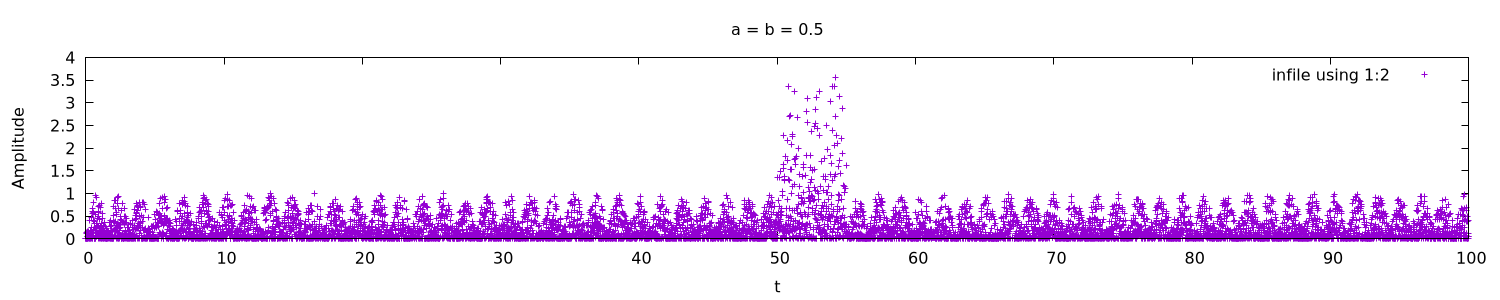
\includegraphics[width=0.98\textwidth]{plots/echo/0.5}
	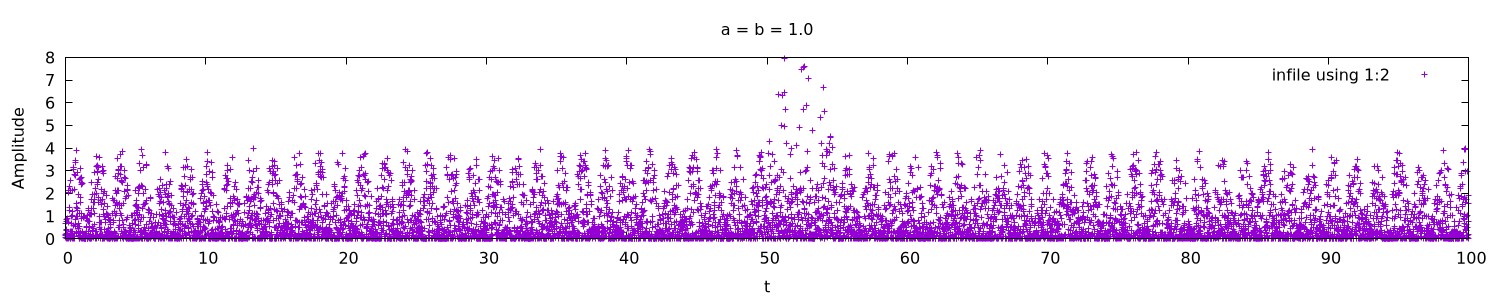
\includegraphics[width=0.98\textwidth]{plots/echo/1.0}
	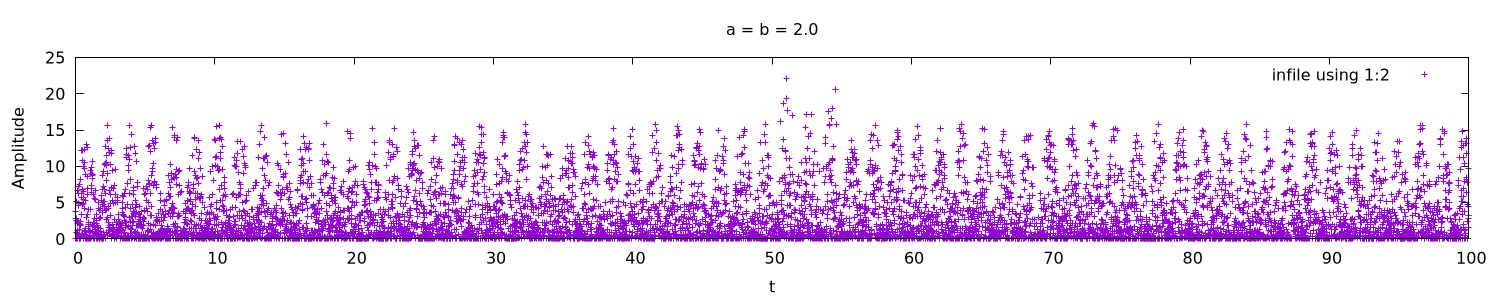
\includegraphics[width=0.98\textwidth]{plots/echo/2.0}
	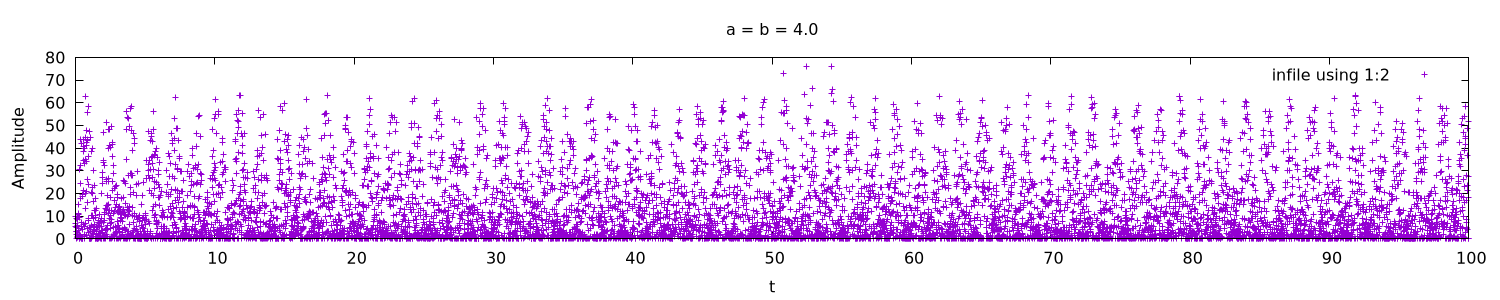
\includegraphics[width=0.98\textwidth]{plots/echo/4.0}
	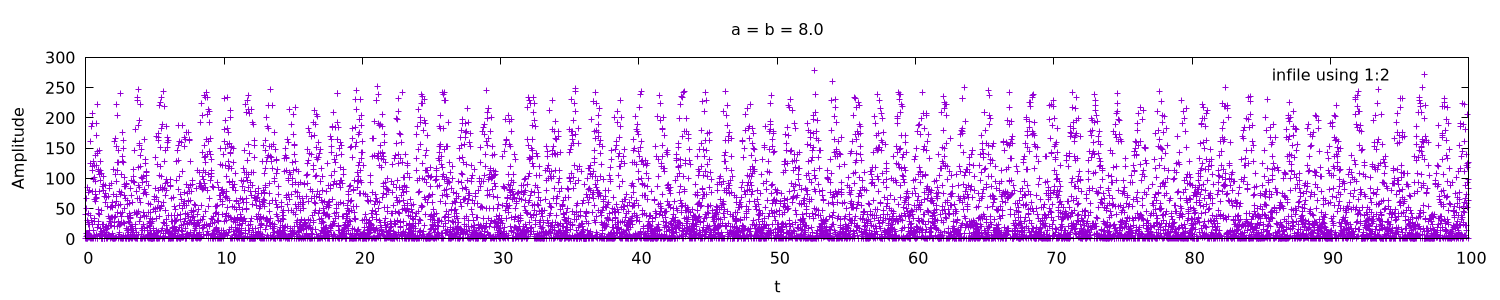
\includegraphics[width=0.98\textwidth]{plots/echo/8.0}
	\caption[$|e(t)|^2$]{Hier ist $|e(t)|^2$ für verschiedene Amplituden $a=b$ dargestellt.}
	\label{fig:2.1}
\end{figure} 
Es lässt sich erkennen, dass für die Amplituden
$a=b=0.5, 1.0$ die Zeit $t_L$ noch sehr gut mit dem Auge abzulesen ist.
Für $a=b=2$ ist es schon schwer die erste Amplitude des Echo-Signals
und damit $t_L$ genau zu identifizieren.
Für $a=b=4$ ist das Signal zwar noch erkenbar aber nur noch auf $\pm3$ einzuschr\"anken.
Für $a=b=8$ ist es quasi nicht mehr möglich das Signal zu erkennen und damit auch nicht möglich $t_L$ abzulesen. 

\subsection{}

In dieser Teilaufgabe soll mit hilfe der Korrelation $(e \odot s)_k$
die Genauigkeit der Bestimmung von $t_L$ verbessert werden.
Datzu stellen wir Gleichung \ref{equ:1.3} nach $(f \odot s)_k$ um:
\begin{equation*}
	(e \odot s)_{k}=\left[\mathcal{F}^{-1}\left( [\mathcal{F} e] \overline{[\mathcal{F} s]}\right)\right]_{k}
\end{equation*}
Diese berechnung sieht im Programm folgendermassen aus:
\begin{lstlisting}[style=CStyle]
	(s.fft() *= e.fft().conj()).rfft()
\end{lstlisting}
Wobei .fft() und .rfft() die FFT und r\"ucktransformationen sind.
Nun haben wir die normierte Korrelation $|(e \odot s)(t)|^{2}$ für die gleichen Störungsamplituden wie in Aufgabe \ref{ssec:10.2} berechnet ($a=b=0.5,1.0 2.0, 4.0, 8.0$) und dargestellt (Abbildung \ref{fig:3.1}).
\begin{figure}[htbp]
	\centering
	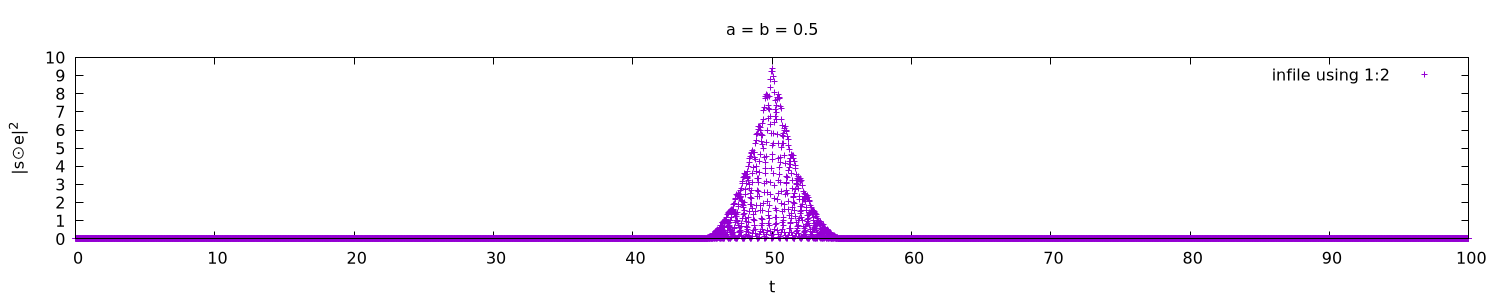
\includegraphics[width=0.98\textwidth]{plots/korrelation/0.5}
	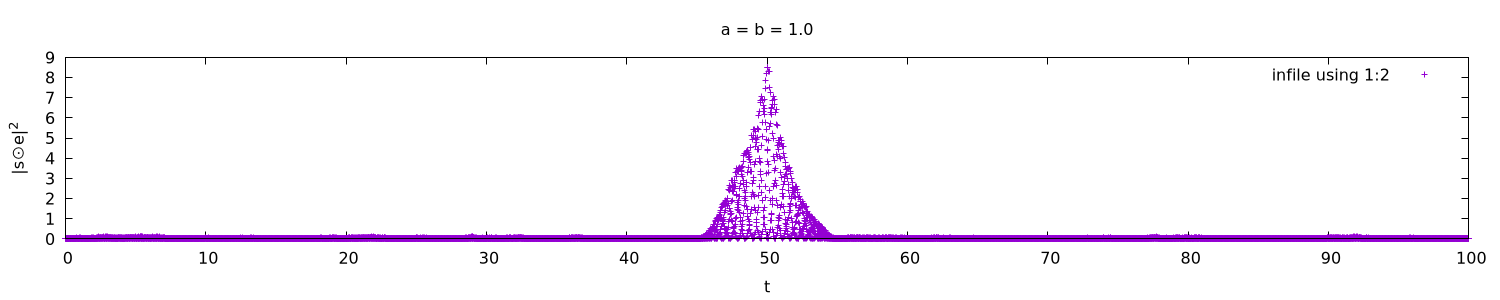
\includegraphics[width=0.98\textwidth]{plots/korrelation/1.0}
	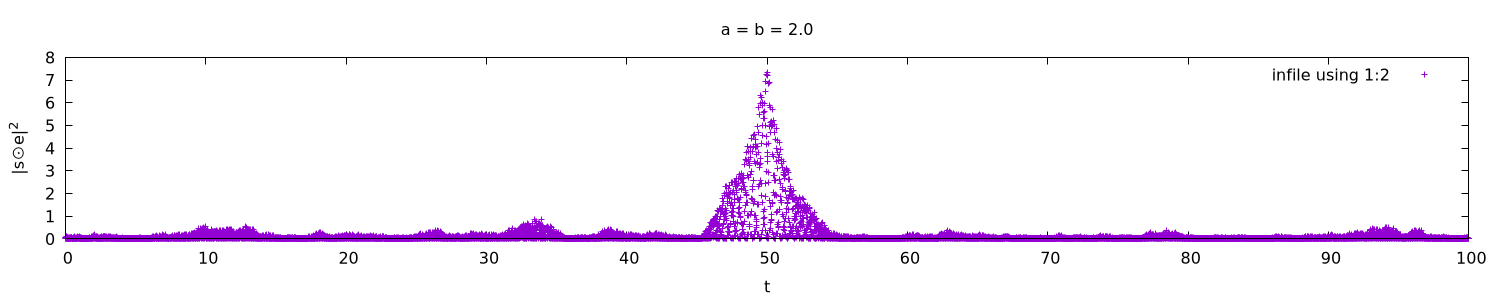
\includegraphics[width=0.98\textwidth]{plots/korrelation/2.0}
	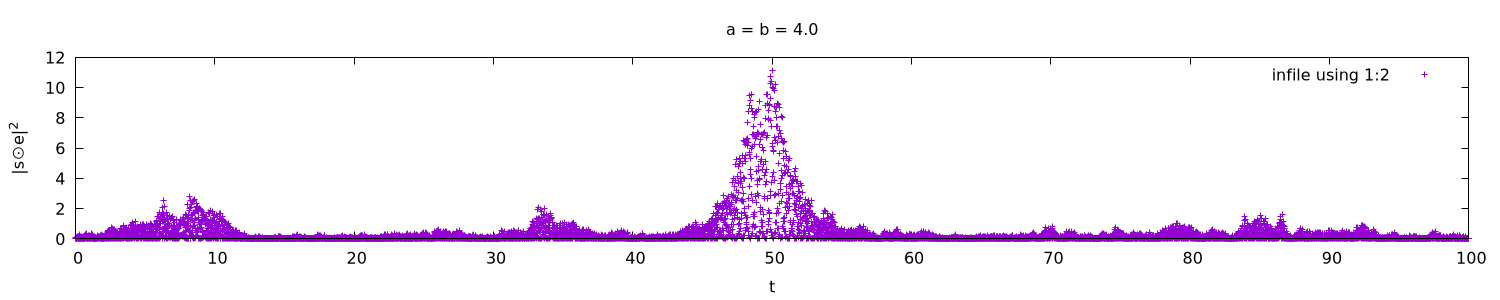
\includegraphics[width=0.98\textwidth]{plots/korrelation/4.0}
	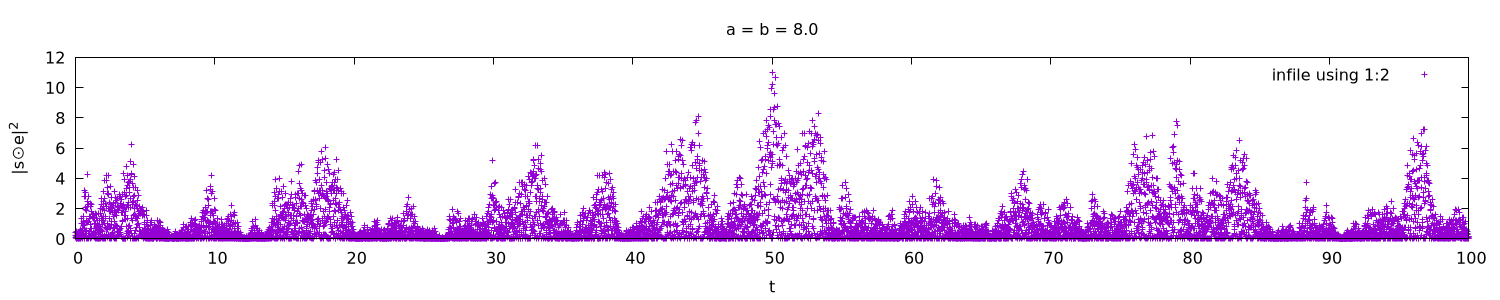
\includegraphics[width=0.98\textwidth]{plots/korrelation/8.0}
	\caption[$|(e \odot s)(t)|^2$]{Hier ist die Korrelation $|(e \odot s)(t)|^2$ für die Amplituden $a=b=0.5, 1.0, 2.0, 4.0, 8.0$ dargestellt.}
	\label{fig:3.1}
\end{figure} 
Mit diesem Verfahren ist es wesentlich einfacher ist $t_L$ zu bestimmen,
da man nur das Maximum der Funktion bestimmen muss.
Dies funktioniert für die Störungsamplituden $a=b=0.5,1,2,4$ sehr gut.
Auserdem ist das verfahren genauer da der peak zu einer spitze l\"auft
die genauer geortet werden kann.
Selbst bei $a=b=8$ ist ein peak noch klar erkenbar. 
\newpage
\subsection{}
Nun betrachten wir die analytische L\"ossung der Korrelation:
\begin{equation*}
	(e \odot s)(t):=\int_{-\infty}^{\infty} \mathrm{d} \tau~ e(t+\tau) s(\tau)
\end{equation*}
Hierbei betrachten wir den st\"orungsfreien Fall $a=b=0$
\begin{align*}
	s(\tau)&=\left\{\begin{array}{ll}
		\sin (2 \pi \alpha \tau) & \text { für } 0 \leq \tau \leq t_{\max } \\
		0 & \text { sonst }
		\end{array}\right.\\
	e(\tau)&=\left\{\begin{array}{ll}
	\sin (2 \pi \alpha (\tau-t_L)) & \text { für } t_L \leq \tau \leq t_L+t_{\max } \\
	0 & \text { sonst }
	\end{array}\right.
\end{align*}
Da  $s(\tau)=0~\forall\tau\notin[0,t_{max}]$ l\"ast sich das Integral umschreiben zu:
\begin{align*}
	(e \odot s)(t):&=\int_{0}^{t_{max}} \mathrm{d} \tau~ e(t+\tau) \sin(2\pi\alpha\tau)\\
	&=\int_{t}^{t+t_{max}} \mathrm{d} \tau~ e(\tau) \sin(2\pi\alpha(\tau-t))\\
\end{align*}
Nun betrachten wir 4 F\"alle:
\begin{itemize}
	\item [(1)] {$\mathbf{t<t_L-t_{max}}$}\\
	In diesem Fall gilt $t+t_{max}<t_L$
	also gilt $e(\tau)=0~\forall\tau\in[t,t+t_{max}]$
	\begin{equation*}
		\Rightarrow(e \odot s)(t)=0
	\end{equation*}
	\item [(2)] {$\mathbf{t_L-t_{max}<t<t_L}$}\\
	In diesem Fall gilt $t<t_L$ und $t+t_{max}<t_L+t_{max}$
	also kann das Integral umgeschrieben werden zu:
	\begin{align*}
		(e ~\odot~ s)(t)&=\int_{t_L}^{t+t_{max}} \mathrm{d} \tau~ \sin(2\pi\alpha(\tau-t_L)) \sin(2\pi\alpha(\tau-t))
	\end{align*}
	Mit dem Additionstheorem: $\sin \alpha \sin \beta = \frac{1}{2} \left[ \cos(\alpha-\beta) - \cos (\alpha+\beta) \right]$
	kann integral umgeschrieben werden zu:
	\begin{align*}
		(e ~\odot~ s)(t)&=\frac{1}{2}\int_{t_L}^{t+t_{max}} \mathrm{d} \tau~ \cos(2\pi\alpha(t-t_L))-\cos(2\pi\alpha(2\tau-t_L-t))\\
		&=\left[\frac{\tau\cos(2\pi\alpha(t-t_L))}{2}-\frac{\sin(2\pi\alpha(2\tau-t_L-t))}{8\pi\alpha}\right]_{\tau=t_L}^{t+t_{max}}\\
		&=\frac{(t+t_{max}-t_L)\cos(2\pi\alpha(t-t_L))}{2}+\frac{\sin(2\pi\alpha(t_L-t))-\sin(2\pi\alpha(2t_{max}+t-t_L))}{8\pi\alpha}
	\end{align*}
	Nun nutzen wir das Additionstheorem $\sin \alpha +\sin \beta = 2 \sin \frac{\alpha + \beta}{2} \cos \frac{\alpha - \beta}{2}$ und kommen auf:
	\begin{equation*}
		(e ~\odot~ s)(t)=\frac{1}{2}\cos(2\pi\alpha(t-t_L))(t_{max}-t_L+t)-\frac{1}{4\pi\alpha}\cos(2\pi\alpha t_{max})\sin(2\pi\alpha(t_{max}-t_L+t))
	\end{equation*}
	\item [(3)] {$\mathbf{t_L<t<t_L+t_{max}}$}\\
	In diesem Fall gilt $t_L<t$ und $t_L+t_{max}<t+t_{max}$
	also kann das Integral umgeschrieben werden zu:
	\begin{align*}
		(e ~\odot~ s)(t)&=\int_{t}^{t_L+t_{max}} \mathrm{d} \tau~ \sin(2\pi\alpha(\tau-t_L)) \sin(2\pi\alpha(\tau-t))
	\end{align*}
	Mit dem Additionstheorem: $\sin \alpha \sin \beta = \frac{1}{2} \left[ \cos(\alpha-\beta) - \cos (\alpha+\beta) \right]$
	kann integral umgeschrieben werden zu:
	\begin{align*}
		(e ~\odot~ s)(t)&=\frac{1}{2}\int_{t}^{t_L+t_{max}} \mathrm{d} \tau~ \cos(2\pi\alpha(t-t_L))-\cos(2\pi\alpha(2\tau-t_L-t))\\
		&=\left[\frac{\tau\cos(2\pi\alpha(t-t_L))}{2}-\frac{\sin(2\pi\alpha(2\tau-t_L-t))}{8\pi\alpha}\right]_{\tau=t}^{t_L+t_{max}}\\
		&=\frac{(t_L+t_{max}-t)\cos(2\pi\alpha(t-t_L))}{2}+\frac{\sin(2\pi\alpha(t-t_L))-\sin(2\pi\alpha(2t_{max}+t_L-t))}{8\pi\alpha}
	\end{align*}
	Nun nutzen wir das Additionstheorem $\sin \alpha +\sin \beta = 2 \sin \frac{\alpha + \beta}{2} \cos \frac{\alpha - \beta}{2}$ und kommen auf:
	\begin{equation*}
		(e ~\odot~ s)(t)=\frac{1}{2}\cos(2\pi\alpha(t-t_L))(t_L-t+t_{max})-\frac{1}{4\pi\alpha}\cos(2\pi\alpha t_{max})\sin(2\pi\alpha(t_{max}+t_L-t))
	\end{equation*}
	\item [(4)] {$\mathbf{t_L+t_{max}<t}$}\\
	Aus $t>t_L+t_{max}$ folgt $e(\tau)=0~\forall\tau\in[t,t+t_{max}]$
	\begin{equation*}
		\Rightarrow(e \odot s)(t)=0
	\end{equation*}
\end{itemize}
Somit haben wir die analytische L\"ossung bestimmt:
\begin{align*}
	&(e ~\odot~ s)(t)=\\
	&\left\{\begin{array}{ll}
	0 & \text { für } t<t_L-t_{max}\\
	\frac{1}{2}\cos(2\pi\alpha(t-t_L))(t_{max}-t_L+t)-\frac{1}{4\pi\alpha}\cos(2\pi\alpha t_{max})\sin(2\pi\alpha(t_{max}-t_L+t))
	& \text { für } t_L-t_{max}<t<t_L\\
	\frac{1}{2}\cos(2\pi\alpha(t-t_L))(t_L-t+t_{max})-\frac{1}{4\pi\alpha}\cos(2\pi\alpha t_{max})\sin(2\pi\alpha(t_{max}+t_L-t))
	& \text { für } t_L<t<t_L+t_{max}\\
	0 & \text { für } t>t_L+t_{max}
	\end{array}\right.
\end{align*}
Diese vergelichen wir in Abilldung \ref{fig:4.1} mit der numerischen L\"ossung.
\begin{figure}[htbp]
	\centering
	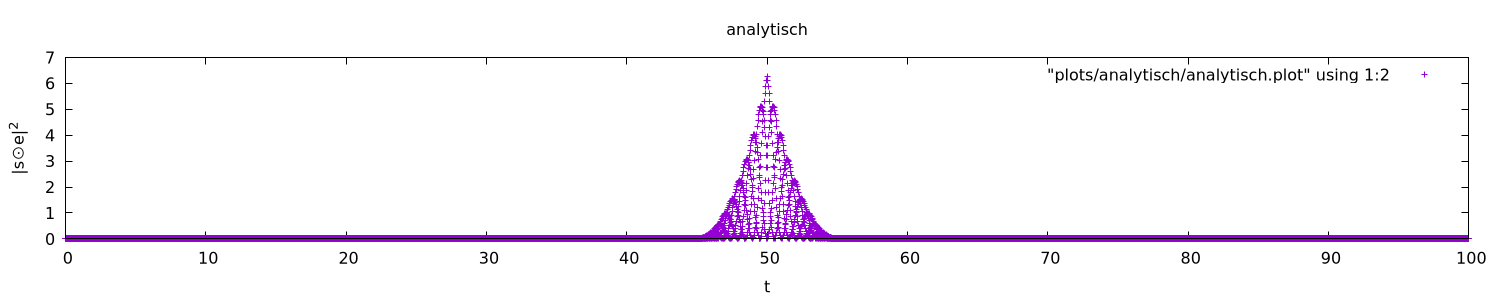
\includegraphics[width=0.98\textwidth]{plots/analytisch/analytisch.png}
	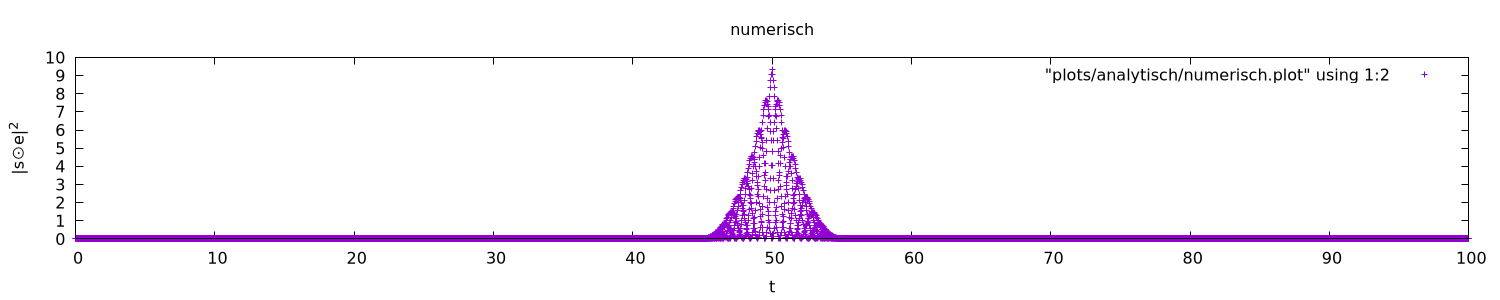
\includegraphics[width=0.98\textwidth]{plots/analytisch/numerisch.png}
	\caption[Vergleich]{Hier haben wir die analytische mit der numerischen Lösung der Korrelation ohne Störung ($a=b=0$) verglichen.}
	\label{fig:4.1}
\end{figure} 
Man sieht das bis auf einen konstanten Vorfaktor diese Funktionen sehr \"ahnlich sind.
Die numerische Funktion dient also zur bestimmung von $t_L$.
\subsection{}
Nun versuchen wir die genauigkeit des Verfahrens zu verbessern.
Datzu nutzen wir einen \emph{Zwitscher}-Puls, welcher eine bessere Autokorrelation aufweist.
Dieser Puls nutzt eine varierende Frequenz um die genaue Verschiebung sch\"arfer zu bestimmen.
Das Signal wird dann beschrieben durch:
\begin{equation*}
s(t)=\left\{\begin{array}{ll}
\sin (2 \pi \alpha(t) t)&,\text { für } 0 \leq t \leq t_{\max } \\
0& ,\text { sonst }
\end{array}\right.
\end{equation*}
In diesem Fall verwenden wir eine lineare Frequenz $\alpha(t)=\alpha_0+t\alpha_1$.
Die resultierenden Korrelationen f\"ur $\alpha_0=5,~\alpha_1=1$ sind in Abilldung \ref{fig:5.1} aufgetragen.

\begin{figure}[htbp]
 	\centering
 	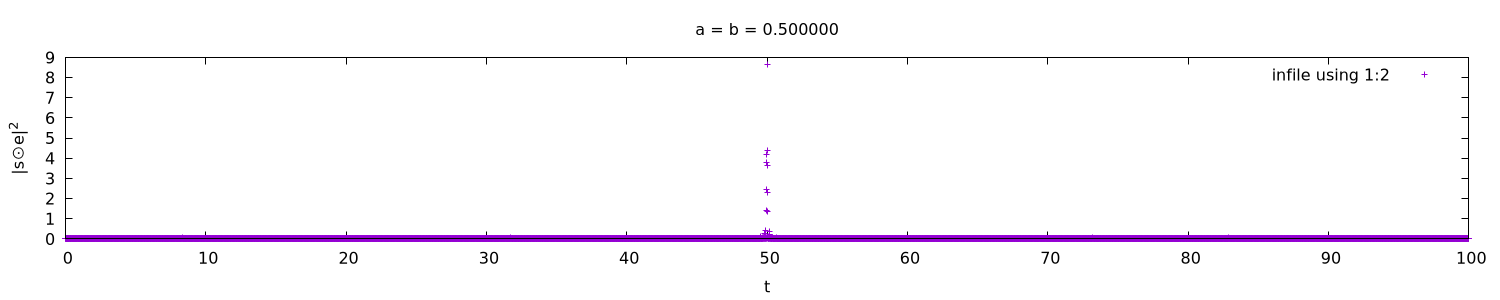
\includegraphics[width=0.98\textwidth]{plots/zwitscher/0.5}
 	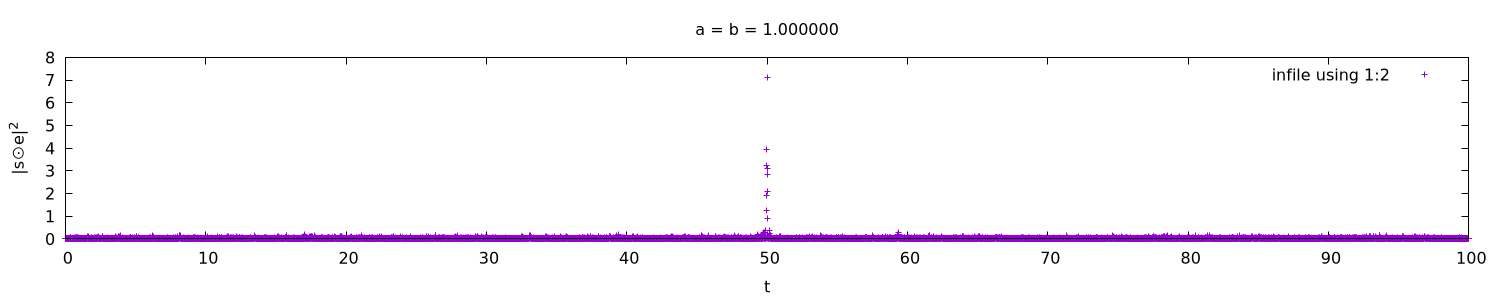
\includegraphics[width=0.98\textwidth]{plots/zwitscher/1.0}
 	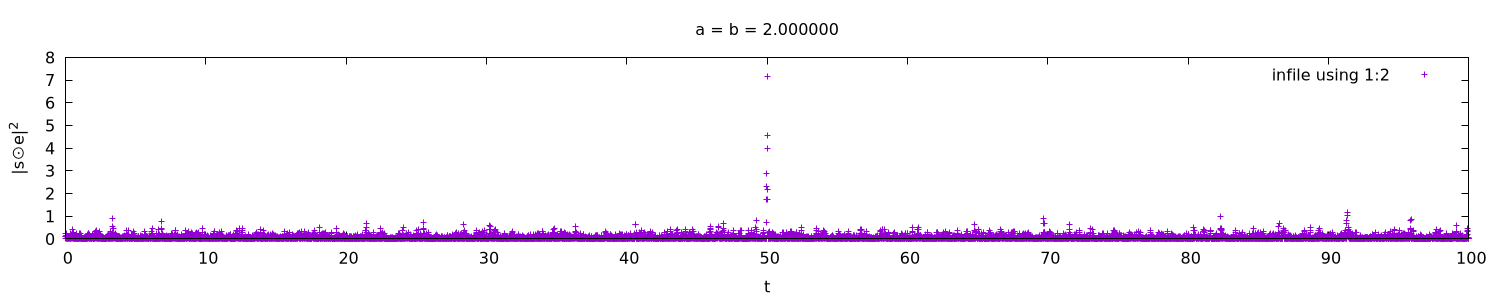
\includegraphics[width=0.98\textwidth]{plots/zwitscher/2.0}
 	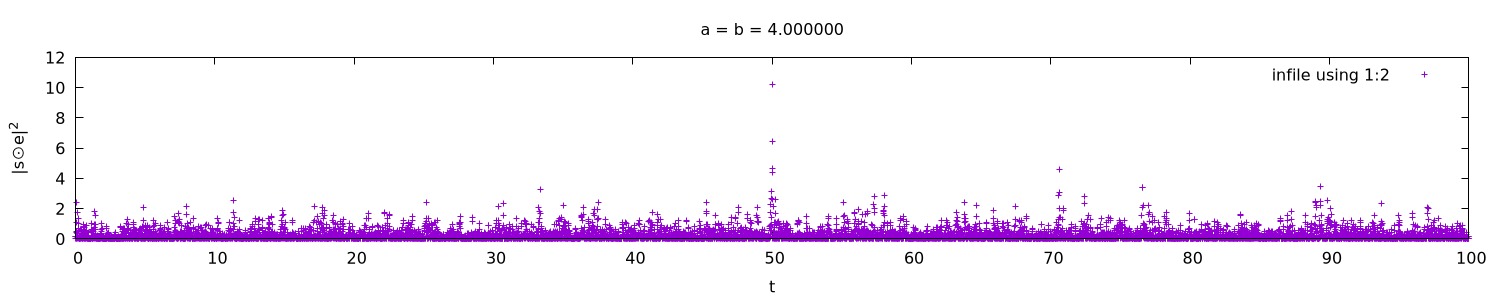
\includegraphics[width=0.98\textwidth]{plots/zwitscher/4.0}
 	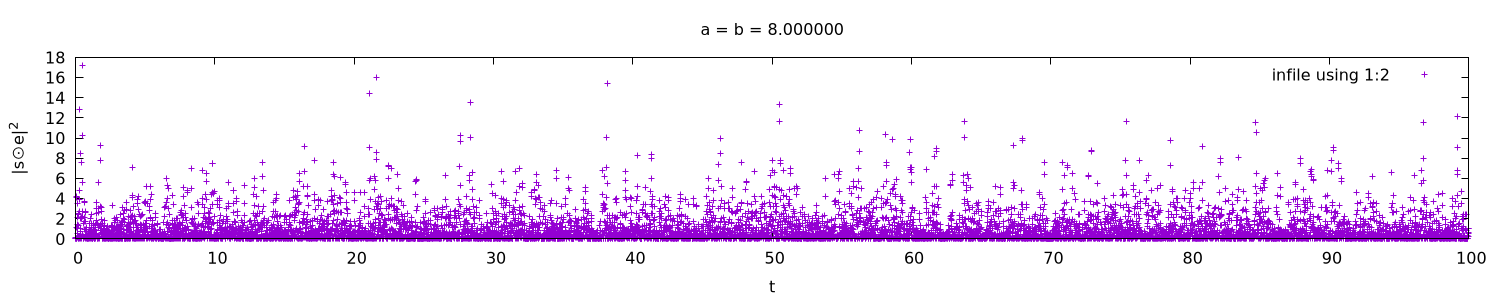
\includegraphics[width=0.98\textwidth]{plots/zwitscher/8.0}
	\caption[$|(e \odot s)(t)|^2$]{Hier ist die Korrelation $|(e \odot s)(t)|^2$ für ein Zwitscher-Signal für die Störamplituden $a=b=0.5, 1.0, 2.0, 4.0, 8.0$ dargestellt.}
	\label{fig:5.1}
\end{figure} 
Das \emph{Zwitscher}-Signal hat die Korrelation sch\"arfer gemacht,
ist aber empfindlicher gegen\"uber grossen St\"orrungen.
\end{document}

